

\section{Discussion}


% ION PAPERS:

% \item{Galy, France-Lanord, Derry: Has the carbonate and silicate rock ratios you can use, including the d13C and d18O}

% \item{Bickle et al, 2015: Rain correction; mass balance calculations to see silicate and carbonate proportions; Modal decomposition for mineral proportions in water.}




% MODELLING:

% \item{Benettin et al, 2015: Develop a transport model for a watershed in the US. Assumptions in modeling approach is that their modelling approach assumes the properties of different compartments are reproduced by the outflow - this suggests that mixing processes and macrodispersion are more important than advective transport}

% \item{Bethke, 2008: The Damkohler number describes the relative importance of reaction and transport, or kinetic vs transport controlled in West's terms}



\subsection{Stoichiometric Considerations}
\begin{itemize}
    \item Matrix example
    \item Feldspar is mostly what we dissolve and kaolinite is mostly what we precipitate
    \item Include the stoichiometry of the reaction from Drever
    \item Decide that at Alakmanda, eg albite component is near 0.8

\end{itemize}

\begin{figure}[h]
    \centering
    \includegraphics[width=\textwidth]{matrix_eg.png}
    \caption{Matrix example of what you need to write}
    \label{fig:discussion5}
\end{figure}

\FloatBarrier


\begin{figure}[h]
    \centering
    \includegraphics[width=\textwidth]{Stoichiometric_eg.png}
    \caption{Example dissolution plot}
    \label{fig:discussion6}
\end{figure}

\FloatBarrier





\subsection{One-Dimensional Reactive Transport Model}


Need to talk about what previous papers have said and how our d18O predicts a particular flow path length eg.

\bsk

Also need to make a mini 1D graphic explaining what the 1D model actually means in practice




\begin{itemize}
    \item Explain the basis behind the model. Maher in that weathering is sensitive to fluid flux moreso than it is to the temperature. Another interpretation is that of Fontorbe where it is sensitive to the temperature.
    \item From same first order differential equation we get two different models
    \item The Maher model because of less constraints the opposite can be used to calculate times for a given rate of reaction, and compare to Abra's already determined ages
    \item Fontorbe we have a series of assumptions that allow us to calculate the rate of reaction which will allow us to determine whether we are close to eqm or not.
    \item The Maher model can also be used to determine the rate of reaction for a given set of concentrations and times
    \item Emphaise how the Maher model wants to predict what weathering is sensitive to

\end{itemize}


\newpage



\subsubsection{Fontorbe Model}

Put the models in boxes?

\bsk

Starts with a first order differential equation describing the reactive transport of Si, assuming reaction rates remain constant along the flow path, which is different from Maher.\\

\begin{equation}
\phi \frac{\partial C}{\partial t} = -\omega \phi \frac{\partial C}{\partial z} + R_n\cdot\left(1-f\right)
\end{equation}\\


Where C is Si concentration, $\phi$ is porosity, $\omega$ is the fluid velocity, z is the distance along the 1D flow path, $R_n$ is the rate of reaction, and f is the fraction of Si reprecipitated in clay minerals. This value is just a function of much Si in the water is precipitated or dissolved. \\

We can then non-dimensionalise, z = hz' where h is the length of the flow path; t= ht'/w, C=CoC' where Co is the initial Si concentration (but can be something else)\\

\begin{equation}
     C' = \frac{C}{C_o} \quad \text{\&} \quad z' = \frac{z}{h} \quad \text{\&} \quad t' = \frac{t\omega}{h}
\end{equation}\\

This transforms the equation 1 to: \\

\begin{equation}
    \frac{\partial C'}{\partial t'} = -\frac{\partial C'}{\partial z'} + N_D\cdot\left(1-f\right)
\end{equation}\\
    

Where \\

\begin{equation}
    N_D = \frac{R_n\cdot h}{\phi\cdot Co \cdot \omega}
\end{equation}\\

Given a quasi-stationary state assumption (Lichtner, 1988), where $\frac{\partial C'}{\partial t'} = 0$, we can solve for the rate of reaction\\

\begin{equation}
    C' = 1 + z' \cdot N_D\cdot\left(1-f\right)
\end{equation} \\

So when z = h, and z' = 1, \\

\begin{equation}
    N_D = \frac{C'_h - 1}{1-f}
\end{equation}\\

Where C' is the concentration of Si at the end of the flow path.\\

We also know that the residence time \( T_f \) is\\

\begin{equation}
T_f = \frac{h}{\omega}
\end{equation}\\

So at the end of the flow path h for a concentration C'$_h$:\\

\begin{equation}
    \frac{R_n\cdot h}{\phi\cdot Co \cdot \omega}  = \frac{C'_h - 1}{1-f}
\end{equation}\\

\begin{equation}
    \frac{R_n\cdot T_f}{\phi\cdot Co \cdot}  = \frac{C'_h - 1}{1-f}
\end{equation}\\

\begin{equation}
    T_f  = \frac{\left(C'_h - 1\right)\cdot\phi\cdot Co}{\left(1-f\right)\cdot R_n}
\end{equation}\\

This can be rearranged for the rate of reaction, $R_c$. It can also be rearranged for time. We get:\\



\begin{equation}
    C'_h = C_h/C_o
\end{equation}\\


\begin{equation}
    T_f  = \frac{\left(C_h - Co\right)\cdot\phi}{\left(1-f\right)\cdot R_n}
\end{equation}\\

Note that this equation leads to times coming out in 10$^{-9}$s, so this needs to be accounted for when converting to years.\\

or

\begin{equation}
    R_n  = \frac{\left(C_h - Co\right)\cdot\phi}{\left(1-f\right)\cdot T_f}
\end{equation}\\

\FloatBarrier
\newpage

\begin{table}[h]
    \centering
    \renewcommand{\arraystretch}{1.3} % Adjust row height
    \begin{tabular}{|c|c|c|c|}
        \hline
        \multicolumn{4}{|c|}{\textbf{Fontorbe}} \\  
        \hline
        \textbf{Parameter} & \textbf{Definition} & \textbf{Units} & \textbf{Formula (Value)} \\  
        \hline
        $\phi$ & Porosity & - & - \\
        $\omega$ & Fluid velocity & m/s & - \\
        $h$ & Length of flow path & m & Variable \\
        $C_h$ & Concentration \@ end of flow path & $\mu$mol/L & Variable \\
        $C_0$ & Initial concentration & $\mu$mol/L & Rain Conc \\
        $f$ & Fraction reprecipitated & - & Order 0.5 \\
        $N_D$ & Non-dimensional number & - & $N_D = \frac{R_n h}{\phi C_0 \omega}$ \\
        $T_f$ & Residence time & $10^{-9}$ s & $T_f = \frac{h}{\omega}$ \\
        $R_n$ & Reaction rate & mol/m$^3$/s & $k\cdot S \cdot \rho \cdot 10^3 \cdot X \cdot (1-\phi) $ \\
        $k$ & Reaction rate constant & mol/m$^2$/s & - \\
        $S$ & Specific surface area & m$^2$/g & - \\
        $\rho$ & Mineral density & kg/m$^3$ &  \\
        $X$ & Volume fraction of mineral in rock & $g_{min}/g_{rock}$ & 0.2 \\
        \hline
    \end{tabular}
    \caption{Key parameters and definitions for the Fontorbe model.}
    \label{tab:parameters1}
\end{table}


\FloatBarrier









\newpage




\subsubsection{Maher Model}


The first order differential equation to solve is:\\ 
\begin{equation}
\frac{dc}{dt} = -\frac{q}{\phi} \frac{dc}{dx} + \sum_{i} \mu_i R_{d,i} \left( 1 - \left( \frac{c}{c_{\text{eq}}} \right)^{n_i} \right)^{m_i} - \sum_{i} \mu_i R_{p,i} \left( 1 - \left( \frac{c}{c_{\text{eq}}} \right)^{n_i} \right)^{m_i}
\end{equation}\\

Where c is the concentration, q is the fluid flux, phi is the porosity

\bsk

Under the quasi-steady state assumption, we can write: \\

\begin{equation}
\frac{dc}{dx} =  \frac{q}{\phi}\sum_{i} \mu_i R_{d,i} \left( 1 - \left( \frac{c}{c_{\text{eq}}} \right)^{n_i} \right)^{m_i} - \frac{q}{\phi}\sum_{i} \mu_i R_{p,i} \left( 1 - \left( \frac{c}{c_{\text{eq}}} \right)^{n_i} \right)^{m_i}
\end{equation} \\

With \\

\begin{equation}
R_n = \sum_{i} \mu_i R_{d,i} - \sum_{i} \mu_i R_{p,i}
\end{equation} \\

Given the definition of \( R_n \) as \\

\begin{equation}
R_n = \sum_{i} \mu_i R_{d,i} - \sum_{i} \mu_i R_{p,i}
\end{equation} \\

Maher and Chamberlain describe that the reaction rate decreases linearly with approach to equilibrium. \\

\begin{equation}
\frac{dc}{dt} = R_n \left( 1 - \frac{c}{c_{\text{eq}}} \right)
\end{equation} \\

Equation 15 can be solved for \( c \), to obtain (following Maher and Chamberlain, 2013)

\begin{equation}
c(x) = c_0 \exp\left(-\frac{R_n \phi x}{q c_{\text{eq}}} \right) + c_{\text{eq}} \left( 1 - \exp\left(-\frac{R_n \phi x}{q c_{\text{eq}}} \right) \right)
\end{equation} \\

We also know that the residence time \( T_f \) is \\

\begin{equation}
T_f = \frac{L\phi}{q}
\end{equation} \\

So \\

\begin{equation}
c(T_f) = c_0 \exp\left(-\frac{R_n T_f}{c_{\text{eq}}} \right) + c_{\text{eq}} \left( 1 - \exp\left(-\frac{R_n T_f}{c_{\text{eq}}} \right) \right)
\end{equation} \\

Following Maher and Chamberlain, 2014, this can be solved and rewritten: \\


\begin{equation}
    C =  \frac{C_{\text{0}}}{1 + \tau D_w / q} + C_{\text{eq}} \frac{\tau D_w / q}{1 + \tau D_w / q}
\end{equation} \\
    
Where \\

\begin{equation}
\tau = e^2; \quad D_w = \frac{L\phi R_n}{C_{\text{eq}}}
\end{equation} \\

This can therefore be rewritten as: \\

\begin{equation}
    C = \frac{C_{\text{0}} + C_{\text{eq}} \cdot T_f\left(e^2 \cdot R_n / C_{\text{eq}}\right)}{1 + T_f\left(e^2 \cdot R_n / C_{\text{eq}}\right)}
\end{equation} \\

The equation can be rearranged for the residence time, \( T_f \), which can be compared to the ages obtained from the Fontorbe model. We get:\\

\begin{equation}
    T_f = \frac{C_{eq} \cdot \left(C - C_0\right)}{e^2 R_n \left( C_{\text{eq}} - C \right)}
\end{equation}\\

Note that this equation leads to times coming out in 10$^{-6}$s, so this needs to be accounted for when converting to years\\

or:\\

\begin{equation}
    R_n = \frac{C_{eq} \cdot \left(C - C_0\right)}{e^2 T_f \left( C_{\text{eq}} - C \right)}
\end{equation}\\





\newpage


\begin{table}[h]
    \centering
    \renewcommand{\arraystretch}{1.3} % Adjust row height
    \begin{tabular}{|c|c|c|c|}
        \hline  % DOUBLE BOLD LINE
        \multicolumn{4}{|c|}{\textbf{Maher}} \\  
        \hline
        \textbf{Parameter} & \textbf{Definition} & \textbf{Units} & \textbf{Formula (Value)} \\  
        $L$ & Length of flow path & m & Variable \\
        $q$ & Flow rate & m/s & Variable \\
        $\phi$ & Porosity & - & 0.3 (but variable) \\
        $R_n$ & Net reaction rate & mol/L/s & $\rho_{sf} \cdot k \cdot A \cdot X_r $ \\
        $\rho_{sf}$ & Mass mineral / Fluid Volume ratio & g/L & $1000 \cdot \rho_b / \phi$ \\
        $\rho_b$ & Plagioclase density & g/cm$^3$ & - \\
        $k$ & Reaction rate constant & mol/m$^2$/s & - \\
        $A$ & Specific surface area & m$^2$/g & 0.1-1 \\
        $X_r$ & Mineral concentration in fresh rock & $g_{min}/g_{rock}$& Wt\% in rock \\
        $\tau$ & Scaling factor & - & $\tau = e^2$ \\
        $D_w$ & Damkohler Coefficient & m$^2$/s & $D_w = \frac{L \phi R_n}{C_{\text{eq}}}$ \\
        $T_f$ & Residence time & $10^{-6}$ s & $T_f = \frac{L \phi}{q}$ \\
        $C_{eq}$ & Equilibrium concentration & $\mu$mol/L & Max Catchment \\
        $C_0$ & Initial concentration & $\mu$mol/L & Rain Conc \\
        \hline
    \end{tabular}
    \caption{Key parameters and definitions for the Maher model.}
    \label{tab:parameters2}
\end{table}


\newpage

\subsubsection{Comparison of the Models}

\begin{table}[h]
    \centering
    \renewcommand{\arraystretch}{2.2} % Adjust row spacing
    \begin{tabular}{cc}
        \toprule
        \textbf{Fontorbe} & \textbf{Maher} \\
        \midrule
        $\displaystyle T_f  = \frac{\left(C_h - C_o\right)\cdot\phi}{\left(1-f\right)\cdot R_n}$ & 
        $\displaystyle T_f = \frac{C_{eq} \cdot \left(C - C_0\right)}{e^2 R_n \left( C_{\text{eq}} - C \right)}$ \\ [10pt]
        $\displaystyle R_n  = \frac{\left(C_h - C_o\right)\cdot\phi}{\left(1-f\right)\cdot T_f}$ & 
        $\displaystyle R_n = \frac{C_{eq} \cdot \left(C - C_0\right)}{e^2 T_f \left( C_{\text{eq}} - C \right)}$ \\
        \bottomrule
    \end{tabular}
    \caption{Comparison of equations from Fontorbe and Maher}
    \label{tab:equations}
\end{table}


From this table comparison, it is easy to see the differences between why the two models will differ in their estimation of residence time.

\bsk

For residence time, both contain the factor - but the RN IS DEFINED DIFFERENTLY TOO \bsk

\[
\frac{C - C_o}{R_n}
\]\\

The difference then comes with the remaining variables in the reaction. For Fontorbe, the porosity divided by the fraction of element reprecipitated makes up the remaining terms. For Maher, the equilibrium concentration divided by the scaling factor and the difference between the equilibrium concentration and the concentration of the element make up the remaining terms.\\

\bsk

Given that both the fraction of element reprecipitated and the scaling factor range between 0-1, the difference in the models will come from the equilibrium concentration in the Maher formula. Indeed, given that the concentration is taken from the highest in the catchment (so as not to follow Maher and Chamberlain (2013)'s rather conservative estiamte following Gaillardet et al. (1999)'s global river data), the fraction \\

\[
\frac{C_{eq}}{C_{eq} - C}
\]\\

will only get larger as the reaction progresses. As the reaction progresses, the Maher model will predict longer times than the Fontorbe model, in the end with two orders of magnitude difference at the older times.\\ 


\begin{figure}[h]
    \centering
    \includegraphics[width=\textwidth]{T_res_Si_uM_EC_comparison.pdf}
    \caption{Comparison for the residence time between the two models. Evaluated for Specific surface area = 0.1; Mineral concentration in rock = 0.36; density of plagioclase = 2.230; Reaction rate constant = 10-15; Porosity = 0.3; Equilibrium concentration = Max in the catchment = 900 uM; Initial concentration = smallest in the traverse; Fraction reprecipitated = 0.5.}
    \label{fig:discussion7}
\end{figure}

\FloatBarrier


\subsubsection{Constraints on Residence Time}

As per Acharya et al. (2020), parts of the literature suggest that the most amount of precipitation occur in the top quarter of the Himalayan catchments. Studies analysing gas ages %(what are they?)
suggest that the residence time of the water in this catchment is on the order of 10 years, with an average of 25 years (Atwood et al, 2020). 

\bsk

Assuming an average rainfall rate of 3.5 m/yr (cite) over the top quarter of the catchment which is approximately 1km long, a m2/yr rate of 3500 is obtained. When considering a 10m wide channel flow of water, a flow rate of 350 m/yr for the top quarter of the catchment is obtained.

\bsk

Secondly, using the oxygen isotopic composition of the springs, and comparing to the rainfall line, it is possible to obtain a flow path length assuming a general slope of 20 degrees:



\begin{figure}[h]
    \centering
    \includegraphics[width=\textwidth]{IMG_1913.pdf}
    \caption{Proving the point that residence time is around 10 years}
    \label{fig:discussion7}
\end{figure}

\FloatBarrier

% \begin{figure}[h]
%     \centering
%     \includegraphics[width=\textwidth]{T_res_DistanceSi_mM_EC.pdf}
%     \caption{Residence time against distance from the ridge crest for the Maher model. Should we do elevation instead?}
%     \label{fig:discussion7}
% \end{figure}

% \FloatBarrier


In this way it is plausible that ~10 years could be how long the water is spending in the cathcment, consistent with the Maher model.

THen you need to talk about Andermann et al, 2013 and the 3 month delay: largely surface flows.




\subsection{Free Energy Calculations}

\begin{itemize}
    \item Delta G can be calulated from the saturation index of the minerals from PhreeQC
    \item Because of the solid solution of feldspar, we have a lowering of delta G as per Dubacq
    \item Compare Delta G against the times obtained from the Maher model. Is maher correct?

\end{itemize}

\begin{figure}[h]
    \centering
    \includegraphics[width=\textwidth]{Albite_histogram.pdf}
    \caption{Histogram of the delta G of albite}
    \label{fig:discussion8}
\end{figure}


\subsubsection{Comparison with Residence Time}




\begin{figure}[h]
    \centering
    \includegraphics[width=\textwidth]{deltag_Albite_kJmol_vs_T_res_Maher_Si_uM_EC.pdf}
    \caption{Comparison of the delta G of albite against the residence time from the Maher model.}
    \label{fig:discussion8}
\end{figure}

\FloatBarrier


\subsubsection{Constraints on Reaction Rate}


If a residence time of 10 years is appropriate, the models can be used to determine the reaction rate. This can then be used to determine whether weathering is sensitive to the fluid flux moreso than it is to the temperature, and that the water particles are close to equilibrium when comparing to the distance from equilibrium.

\bsk

With a residence time of 10 years, it is possible to see what the reaction rate is using the following relationship: \\

\begin{equation}
    R_n = \frac{C_{eq} \cdot \left(C - C_0\right)}{e^2 T_f \left( C_{\text{eq}} - C \right)}
\end{equation}\\

\begin{equation}
    \rho_{sf} \cdot k \cdot A \cdot X_r = \frac{C_{eq} \cdot \left(C - C_0\right)}{e^2 T_f \left( C_{\text{eq}} - C \right)}
\end{equation}\\


\begin{equation}
     k = \frac{C_{eq} \cdot \left(C - C_0\right)}{e^2 T_f \left( C_{\text{eq}} - C \right) \cdot \rho_{sf} \cdot A \cdot X_r}
\end{equation}\\

Taking the range of samples that correspond to MKS-5 to MKS-9, the places where Atwood et al, 2020 took their lowest elevation sample and found a time of 13 years, we can calculate the reaction rate constant, and compare it to the delta g assuming a simple increase in time with the samples. Note that the time Atwood found for their samples did not ascribe to this simple linear decrease, nor do we expect the time to do so. But for a proof of concept it should demonstrate how the rates of reaction plot:\\


\begin{figure}[h]
    \centering
    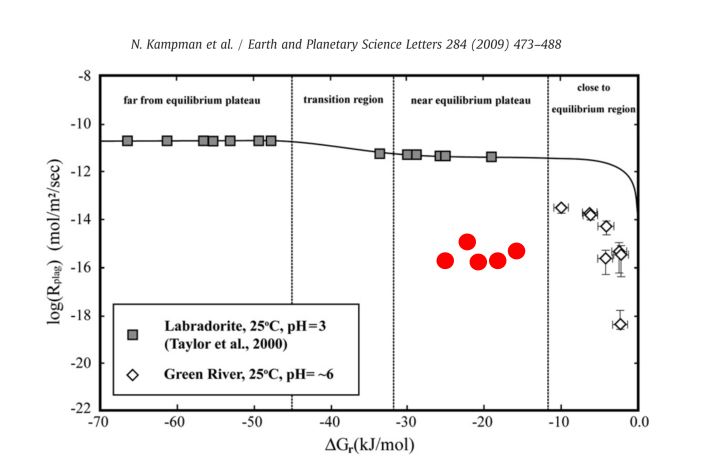
\includegraphics[width=\textwidth]{example_rate_deltaG.pdf}
    \caption{Proving the point that the reaction rate is 10-15.}
    \label{fig:discussion7}
\end{figure}

\FloatBarrier

It is clear from this plot that the obtained reaction rate is of the order of 10$^{-15}$ mol/m2/s. However unlike it does not show a decrease that we would expect if the system was truly approaching equilibrium. Indeed the delta G is still in Kampman's "near equilibrium plateau". And there is still a ways to go before the system is truly close to equilibrium. Insert sentence about obviously Kampman is a different system but the point is that the system is not close to equilibrium.\\

\bsk

So Maher's model for this natural system is not apt in showcasing that 







\FloatBarrier


